\documentclass[a4paper,11pt]{article}
\usepackage[czech]{babel}
\usepackage[left=2cm,text={17cm,24cm},top=3cm]{geometry}
\usepackage[hidelinks]{hyperref}
\usepackage[utf8]{inputenc}
\usepackage[T1]{fontenc}
\usepackage{listings}
\usepackage{xcolor}
\usepackage[perpage]{footmisc}
\usepackage{graphicx}

\graphicspath{ {./resources/} }

\definecolor{gray}{rgb}{0.95,0.95,0.95}
\definecolor{darkred}{rgb}{0.545,0,0}

\title{Dokumentace k projektu z ISA \\
        \large Tunelování datových přenosů přes DNS dotazy}

\author{Hung Do \\ \href{mailto:xdohun00@stud.fit.vutbr.cz}{xdohun00@stud.fit.vutbr.cz}}

\begin{document}
    \maketitle
    \thispagestyle{empty}
    \newpage
    \tableofcontents
    \newpage
    \section{Úvod}
    \subsection{Domain Name System}
    \textbf{DNS} neboli \textbf{Domain Name System} slouží pro převod doménových jmen do IP adres uzlů v síti.
    Jde o decentralizovaný, hierarchický systém doménových jmen, který je uspořádán do stromové struktury.
    Každý uzel stromu může mít pod sebou seznam podřízených domén. V kořeni tohoto stromu se nachází \emph{tečka}.
    Pod ní se nachází \emph{domény nejvýšší úrovně} (např. com, cz, sk, apod.). A tato hierarchie pokračuje dále.

    Strom se dá rozdělit do jednotlivých zón, které spravují správci daných zón.
    \subsection{DNS tunel}
    \textbf{DNS tunelování} patří mezi znáné kyberútoky. Využívá toho, že většina systémů mají povolený protokol
    DNS. Utočník si vytvoří cílovou doménu, která musí být viditelná externě. Následně pomocí např. trojského koně
    zakóduje data souborů či jiných programů do DNS dotazů a ten se odešle na útočníkův autorativní DNS server.
    Tam se data složí do své původní podoby.\cite{DnsTunnel}

    \section{Návrh implementace}
    \begin{figure}[h!]
        \centering
        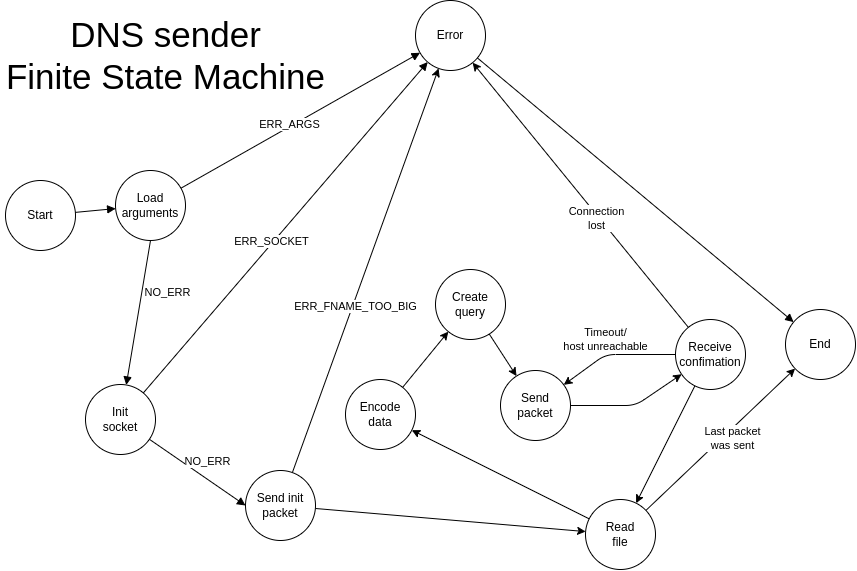
\includegraphics[width=400pt]{sender_fsm}
        \caption{Konečný automat programu \textbf{dns\_sender}}
    \end{figure}
    \begin{figure}[h]
        \centering
        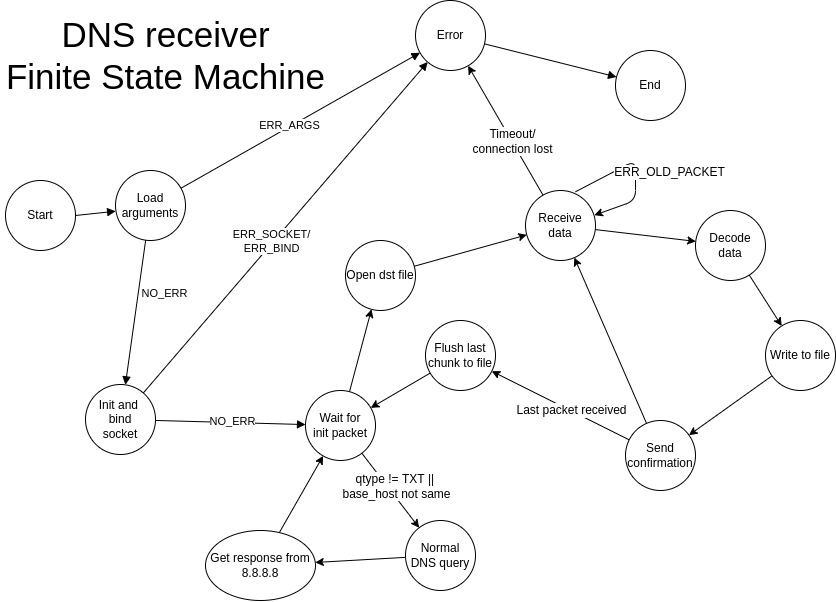
\includegraphics[width=400pt]{receiver_fsm}
        \caption{Konečný automat programu \textbf{dns\_receiver}}
    \end{figure}
    \begin{figure}[h]
        \centering
        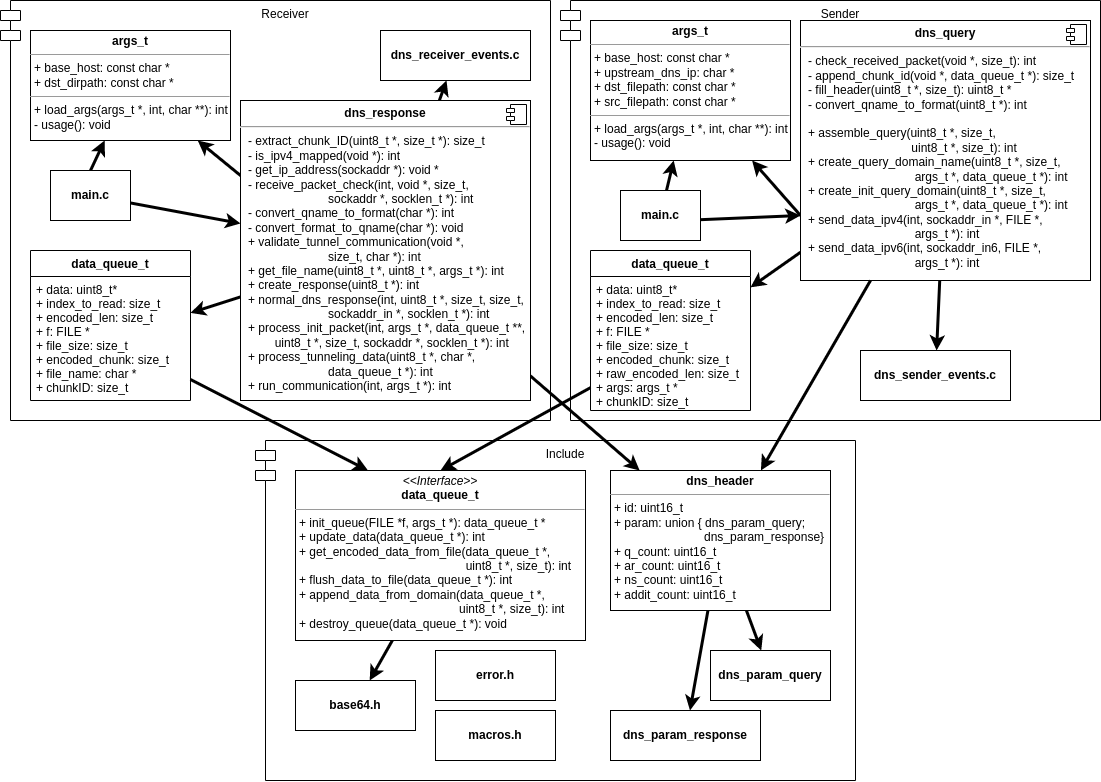
\includegraphics[width=\textwidth]{module_diagram}
        \caption{Propojení jednotlivých modulů v projektu}
    \end{figure}
    \clearpage

    \section{Implementace}
    \label{sec:implementace}
    Implementace projektu je realizována v programovacím jazyce C za použití systémových knihoven
    \verb|<arpa/inet.h>|, \verb|<netinet/in.h>| a \verb|<sys/socket.h>|. Pro algoritmus kódování
    base64 byly použité zdrojové soubory od \textbf{The Apache Group}\footnote{Zdrojové soubory jsou k nalezení \href{https://opensource.apple.com/source/QuickTimeStreamingServer/QuickTimeStreamingServer-452/CommonUtilitiesLib/}{\textbf{zde}}.}.

    \subsection{DNS Sender}
    Implementace \verb|dns_sender| se nachází ve složce \verb|sender/|. Program je rozdělen do čtyř částí:
    \begin{itemize}
        \setlength\itemsep{1pt}
        \item \verb|main|       \-- startující bod programu; vytváří a nastavuje soket
        \item \verb|dns_query|  \-- načítá, kóduje, transformuje a odesílá data na server
        \item \verb|arguments|  \-- zpracovává argumenty programu
        \item \verb|data_queue| \-- definice struktury pro uchování zakódovaných dat a dalších pomocných informací
    \end{itemize}
    V souboru \verb|main.c| se vytváří a nastavují sokety pro komunikaci. Po nastavení soketů se zavolá funkce
    \verb|send_data| z \verb|dns_query.h|, která již zpracovává, transformuje a odesílá data na server. Jádrem programu
    je soubor \verb|dns_query.c|, který obsahuje funkce potřebné pro tvorbu DNS dotazů.

    Komunikace začíná inicializačním paketem, který definuje jméno cílového souboru \emph{DST\_FILEPATH} a
    první \emph{chunkID} komunikace. Po úspěšném navázání kontaktu ve odesílají DNS dotazy s daty.
    Paketu je nejprve nastavena výchozí DNS hlavička, poté se vygeneruje doménové jméno. Doménové jméno je ve formátu:
    \begin{verbatim}
        [chunkID].[collection_of_labels].[base_host] \end{verbatim}
    Jednotlivé \emph{labels} jsou naplňovány zakódovanými daty získané ze souboru \emph{SRC\_FILEPATH} (viz. sekce \ref{sec:SenderUsage}).
    Po odeslání a přijmutí posledního paketu vypíše program ukončující log a ukončí úspěšně program.

    \subsection{DNS Receiver}
    Zdrojové soubory k \verb|dns_receiver| jsou k nalezení ve složce \verb|receiver/|. Obdobně jako \verb|dns_sender| je rozdělen
    do čtyř částí:
    \begin{itemize}
        \setlength\itemsep{1pt}
        \item \verb|main|           \-- startující bod programu; vytváří a nastavuje soket
        \item \verb|dns_response|   \-- přijímá dotazy, dešifruje obsah paketů a skládá z dat cílový soubor
        \item \verb|arguments|      \-- zpracovává argumenty programu
        \item \verb|data_queue|     \-- definice struktury pro uchování zakódovaných dat a dalších pomocných informací
    \end{itemize}
    Příjemce dat je čeká na inicializační paket, ze kterého dešífruje jméno cílového souboru. Do něj se ukládají dešifrovaná data
    příjimaných dotazů. Cyklus se načítá do doby, než server obdrží dotaz na doménu, která je kratší než nejdelší povolené jméno\footnote{Formát je definován zde: \url{https://datatracker.ietf.org/doc/html/rfc1035\#section-2.3.4}}.
    Po dokončení program čeká na další spojení není-li definováno jinak (viz. sekce \ref{ReceiverMode}).

    \subsection{Data Queue struktura}
    Tato struktura je sdílená v obou programech a její obsah je definována každým programem jinak.
    Jedná se o pomocnou strukturu, která obsahuje pomocná data (např. jméno cílového souboru či hodnota \emph{chunkID})
    a do které si program ukládá zakódovaná data. Jednotlivé struktury jsou definované v souborech
    \verb|sender/send_queue.h| resp. \verb|receiver/recv_queue.h|.

    \verb|dns_sender| ze struktury
    odebírá data a vkládá je do jednotlivých \emph{labels}. Pokud již z fronty odebral všechny data, struktura
    automaticky načte nová data ze zdrojového souboru a zakódovaná data vloží opět do fronty.

    \verb|dns_receiver| naopak strukturu naplňuje přijímanými daty z DNS dotazů. Pokud se fronta naplní, struktura
    dešifruje obsah fronty a data \uv{spláchne} do cílového souboru.

    \subsection{Chybové kódy}
    Chybové kódy jsou definované v souboru \verb|include/error.h|.
    \begin{itemize}
        \setlength\itemsep{1pt}
        \item \verb|NO_ERR|            (0) \-- nenastala žádná chyba
        \item \verb|ERR_ARGS|          (1) \-- uživatel nezadal všechny povinné argumenty programu
        \item \verb|ERR_SOCKET|        (2) \-- nepovedlo se vytvořit soket
        \item \verb|ERR_IP_FORMAT|     (3) \-- špatný format IP adresy (IPv4 i IPv6)
        \item \verb|ERR_CONNECT|       (4) \-- nepovedlo se vytvořit spojení mezi klientem a serverem
        \item \verb|ERR_NO_FILE|       (5) \-- zdrojový souboru nebyl nalezen
        \item \verb|ERR_BIND|          (6) \-- nepodařilo se připojit soket k portu
        \item \verb|ERR_FNAME_TOO_BIG| (254) \-- jméno cílového souboru je moc dlouhý a není možno vytvořit inicializační paket
    \item \verb|ERR_OTHER|         (253) \-- předem nepředvídatelná chyba (např. nepovedená alokace paměti)
    \end{itemize}

    \subsection{Zajímavé pasáže kódu}
    Pro zefektivnění přenosu dat, \verb|dns_sender| se snaží odeslat co nejvíce dat skrze jeden DNS dotaz.
    Pomocí jednoduché funkce \verb|MIN(a,b)|, která vrací nižší hodnotu ze 2, dokáže zjistit, kolik bajtů
    může do dotazu ještě vložit, aby nepřesáhla maximální povolenou velikost \emph{label} a přitom neobsadilo místo
    vyhrazenou pro \verb|BASE_HOST|.
    \begin{lstlisting}[language=C,
                       backgroundcolor=\color{gray},
                       keywordstyle=\color{darkred},
                       commentstyle=\color{blue},
                       basicstyle=\ttfamily\footnotesize,
                       breaklines=true,
                       showstringspaces=false]
/* dns_query.c */
int create_query_domain_name(uint8_t *buffer, size_t buffer_size,
        struct args_t *args, struct data_queue_t *q) {
    // ...

    // reset buffer
    memset(buffer, 0, buffer_size);
    static uint8_t label[LABEL_SIZE] = { 0, };
    // secondary buffer for pointer arithmetics
    uint8_t *buffer_ptr = buffer + 1;

    // append chunk ID
    size_t chunk_size = append_chunk_id(buffer_ptr, q);
    buffer_ptr += chunk_size;

    size_t len, total = 0;
    size_t available_size = buffer_size - strlen(args->base_host)
                                - 2 - buffer[0] - chunk_size;

    // cycle to fill labels
    while ((len = get_encoded_data_from_file(q, label,
                    MIN(LABEL_SIZE,available_size - total))) == LABEL_SIZE) {
                //  ^^^^^^^^^^^^^^^^^^^^^^^^^^^^^^^^^^^^^^^
        // move data from label into destination buffer
        memcpy(buffer_ptr + total, label, len);
        total += len;
        q->raw_encoded_len += len;
        q->encoded_chunk += len;
        // append separator
        buffer_ptr[total++] = '.';
    }
    // append last label
    memcpy(buffer_ptr + total, label, len);
    total += len;
    q->raw_encoded_len += len;
    q->encoded_chunk += len;

    // add separator and append domain
    buffer_ptr[total] = '.';
    memcpy(buffer + total + 2 + chunk_size,
           args->base_host, strlen(args->base_host));

    // ...
}
    \end{lstlisting}

    \section{Základní informace o programu}
    Program \verb|dns_receiver| podporuje komunikaci jak pomocí IPv4, tak i IPv6 protokolů. Ke komunikaci bylo použitý protokol UDP.
    Ztráta paketu je ošetřena pomocí nastavení soketu odesílatele. Ten paket může poslat maximálně 5x
    po 3 sekundových intervalech. V případě, že i pátý paket nebyl úspěšně doručen, je program terminován.

    Poté, co příjemce dat vytvoří spojení s odesílatelem, je mu nastavený \emph{timeout} pro čekání na odeslaná data.
    Pokud příjemce nedostane do 15 sekund žádný paket a neobdržel poslední ukončující paket, prohlásí spojení za ztracené a
    ukončí program. \verb|dns_receiver| umí též odpovědět na klasické DNS dotazy. Pokud přijatý dotaz nesplňuje dohodnutý format
    tunelovacího paketu (viz. sekce \ref{sec:implementace}), dotaz je automaticky přesměrován na veřejný Google DNS server
    na adrese \textbf{8.8.8.8}. Odpověď z Google serveru je poté zase přesměrovaná zpátky odesílateli.

    \label{ReceiverMode}
    V souboru \verb|include/macros.h| se nachází makro \verb|CONTINUOUS_RUNNING|, skrze který je možno definovat mód programu \verb|dns_receiver|.
    Pokud je hodnota makra nastavena na 0, program se ukončí, jakmile úspěšně dokoná přenos programu/vyřízení DNS dotazu. V opačném
    případě program bězí, dokud nenastane chyba (ztráta spojení) či je násilně ukončen (např. SIGSEGV).
    Po změně hodnoty je potřeba znovu přeložit program (\verb|make clean && make|).

    \section{Návod na použití}
    Pro vytvoření komunikace mezi oběma programy je zapotřebí, aby strana simulující server měla \textbf{sudo oprávnění} a
    volný \textbf{DNS port (port 53)}. Pokud je port již zabraný, je možný ho uvolnit pomocí programu
    \verb|fuser|\footnote{viz. manuálové stránky: \url{https://man7.org/linux/man-pages/man1/fuser.1.html}}. Druhá možnost je
    přerušení procesu vyžadující daný port.
    \begin{verbatim}
[root@fedora ~]# ss -naup | grep ":53 "
UNCONN 0      0                         127.0.0.53%lo:53         0.0.0.0:*
    users:(("systemd-resolve",pid=945,fd=17))
[root@fedora ~]# systemctl stop systemd-resolved.service
[root@fedora ~]# ss -naup | grep ":53 "
[root@fedora ~]#\end{verbatim}
    Poté, co máme zajištěný port 53, je možné komunikaci rozjet.

    \noindent
    Na serveru rozjedeme program \verb|dns_receiver|. Parametry programu \verb|dns_receiver| jsou:
    \begin{itemize}
        \item \verb|BASE_HOST| \-- definuje útočníkovu (cílovou) doménu, na kterou se odesílají data
        \item \verb|DST_DIRPATH| \-- definuje cílovou složku, do které se mají vytvářet soubory s přijímanými daty.
        Pokud složka neexistuje, je programem vytvořena.
    \end{itemize}

    \noindent
    \label{sec:SenderUsage}
    Na straně klienta rozjedeme program \verb|dns_sender|. Parametry programu \verb|dns_sender| jsou:
    \begin{itemize}
        \item \verb|-u UPSTREAM_IP| \-- definuje, na jakou IP adresu má program přesměrovat DNS dotazy.
        Pokud toto nastavení není definované, program načte adresu ze souboru \verb|/etv/resolve.conf|.
        \item \verb|BASE_HOST| \-- definuje cílovou doménu (musí být stejná jako zadaná ve \verb|dns_receiver|).
        \item \verb|DST_FILEPATH| \-- definuje jméno cílového souboru (jak se bude jmenovat soubor uložený na útočníkově straně).
        \item \verb|SRC_FILEPATH| (volitelný) \-- definuje cestu ke zdrojovému souboru. Pokud zdrojový soubor nebyl zadán,
        program naslouchá ze \verb|STDIN|.
    \end{itemize}

    K překladu projektu slouží přiložený souboru \verb|./Makefile| (více informací naleznete v \verb|README.md|). Příklady rozjetí komunikace naleznete v sekci \ref{sec:testovani}.

    \section{Testování}
    \label{sec:testovani}
    Na testování byly použité 2 systémy:
    \begin{itemize}
        \item \verb|Manjaro Linux x86_64|, s jádrem \verb|5.15.32-3-MANJARO|.
        \item \verb|Fedora Server x86_64|, s jádrem \verb|5.17.12-100.fc34.x86_64|
    \end{itemize}

    Z prvního systému se zapínal program \verb|dns_sender| a odesílaly se z něj data.
    Druhý systém zprávu přijímal a data skládal do souboru pomocí programu \verb|dns_receiver|.

    \noindent
    \begin{figure}[h]
        \centering
        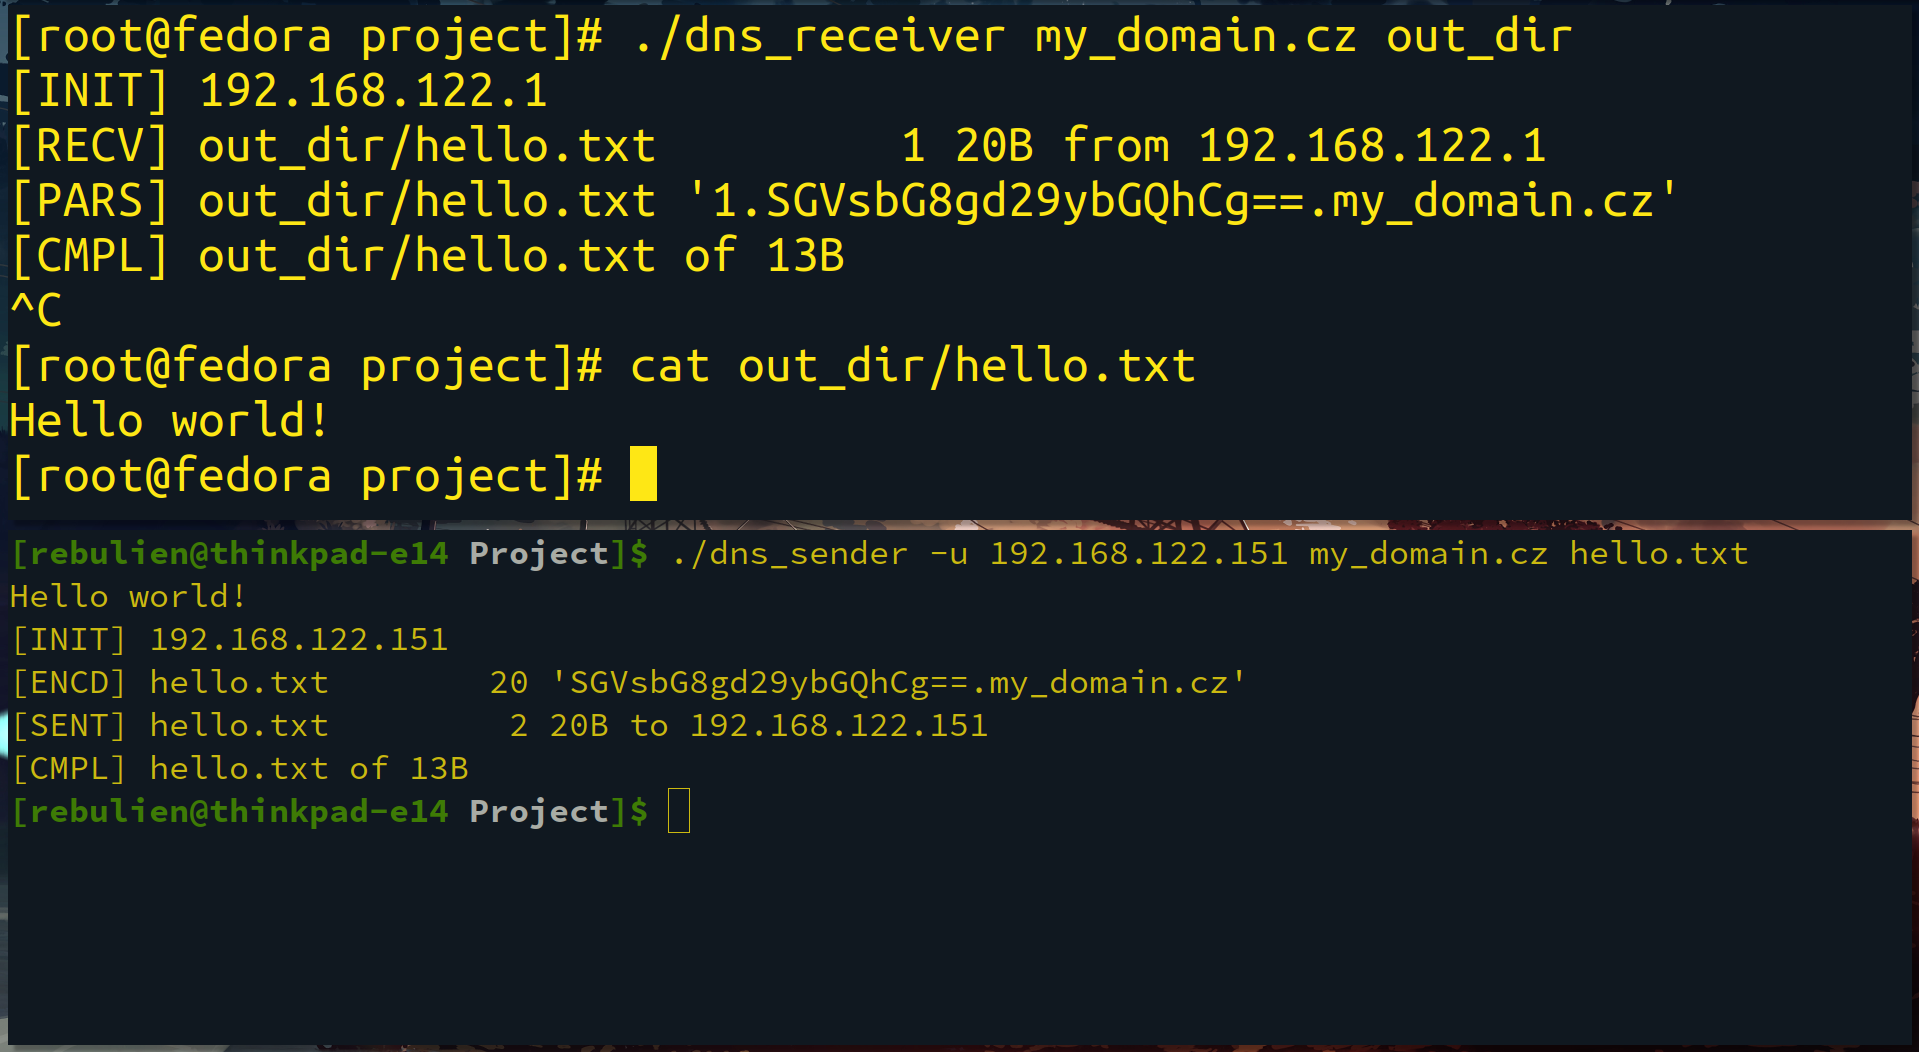
\includegraphics[width=300pt]{simple_text}
        \caption{Odesílání dat ze \emph{STDIN}}
    \end{figure}
    \noindent
    \begin{figure}[h]
        \centering
        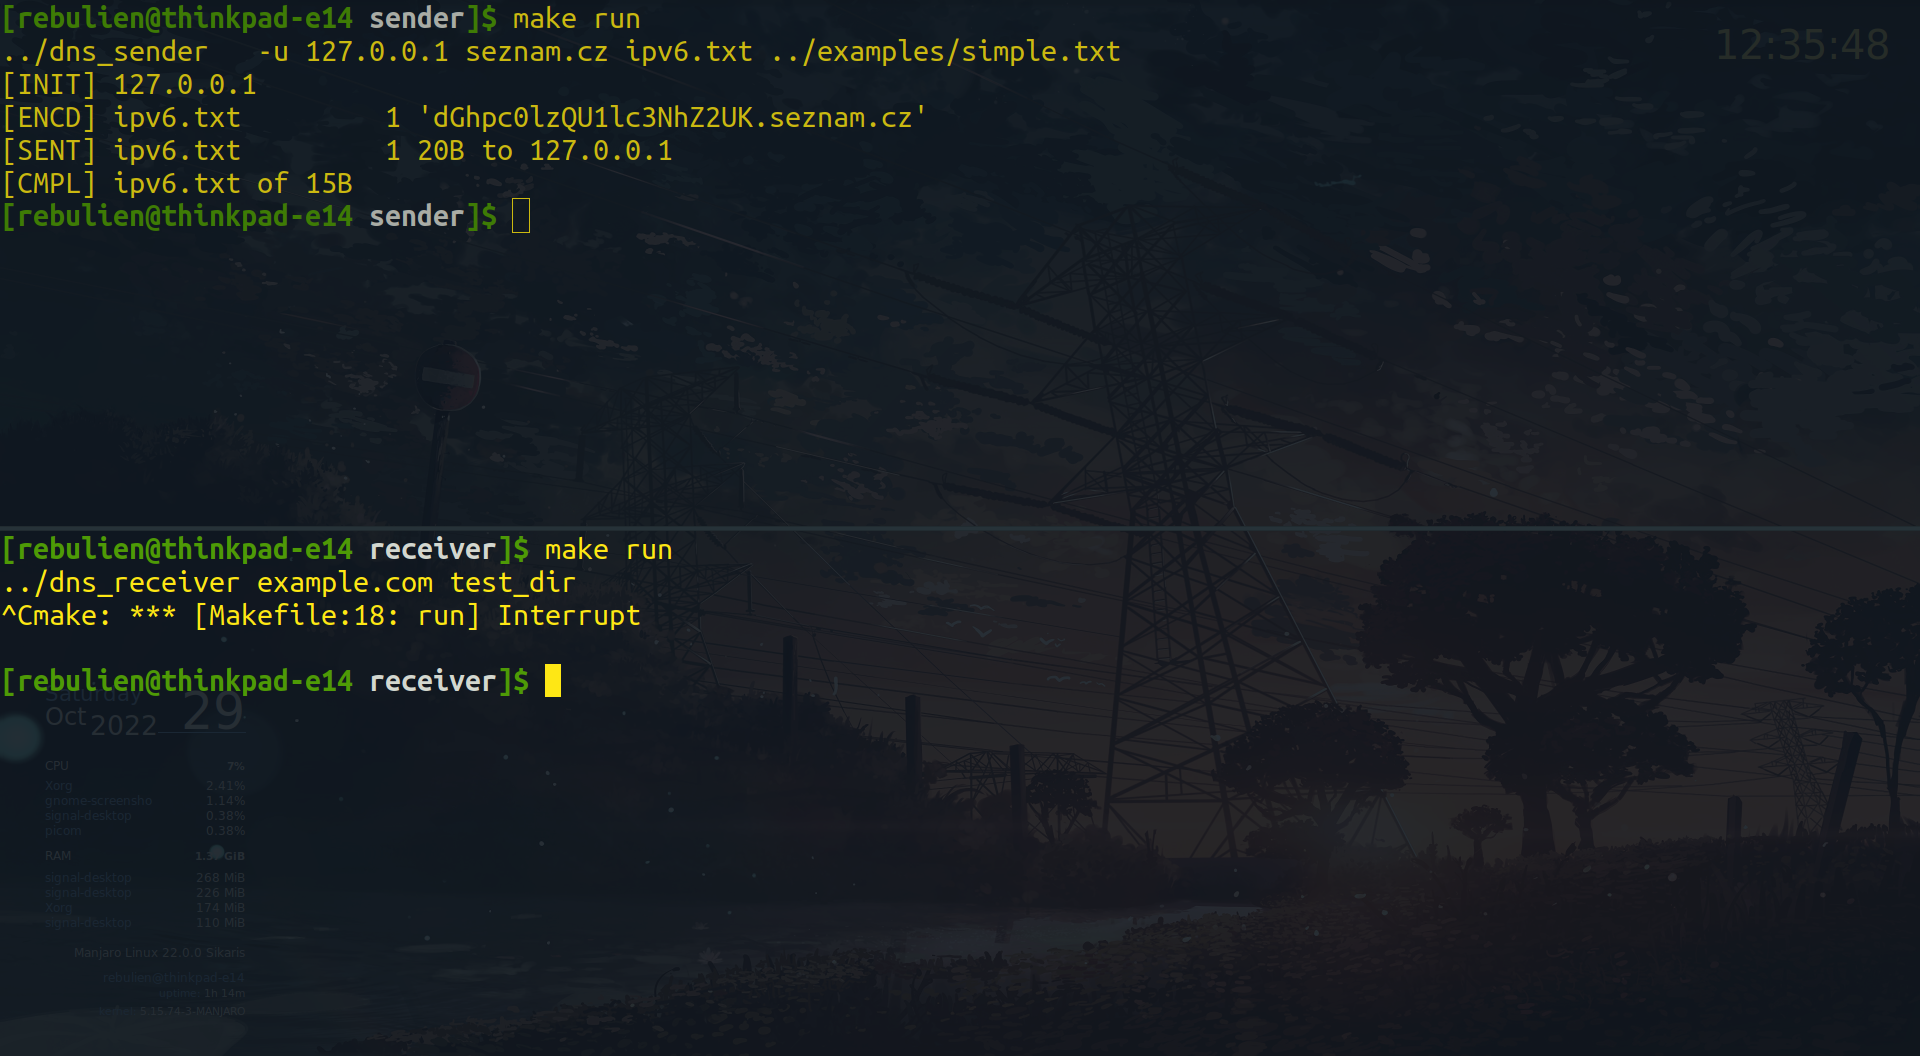
\includegraphics[width=250pt]{normal_query}
        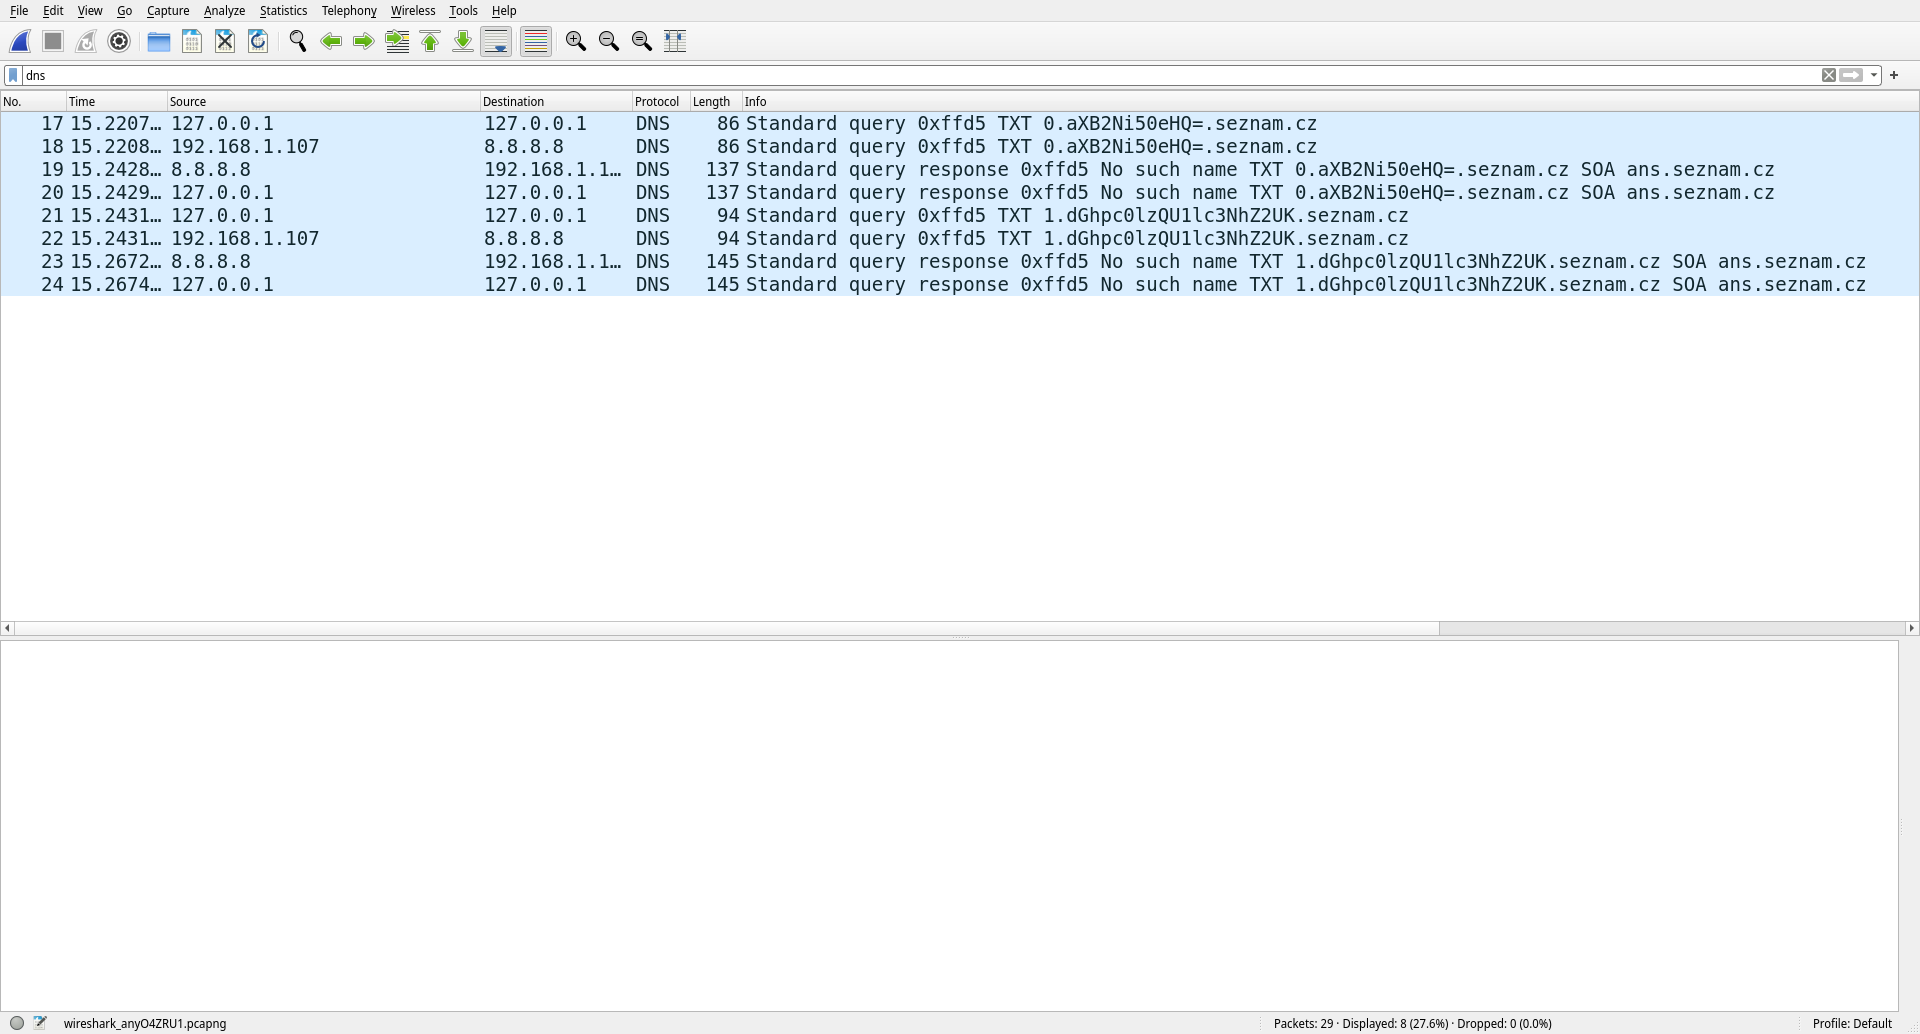
\includegraphics[width=250pt]{wireshark}
        \caption{Odesílání normálního DNS dotazu}
    \end{figure}
    \noindent
    \begin{figure}[h]
        \centering
        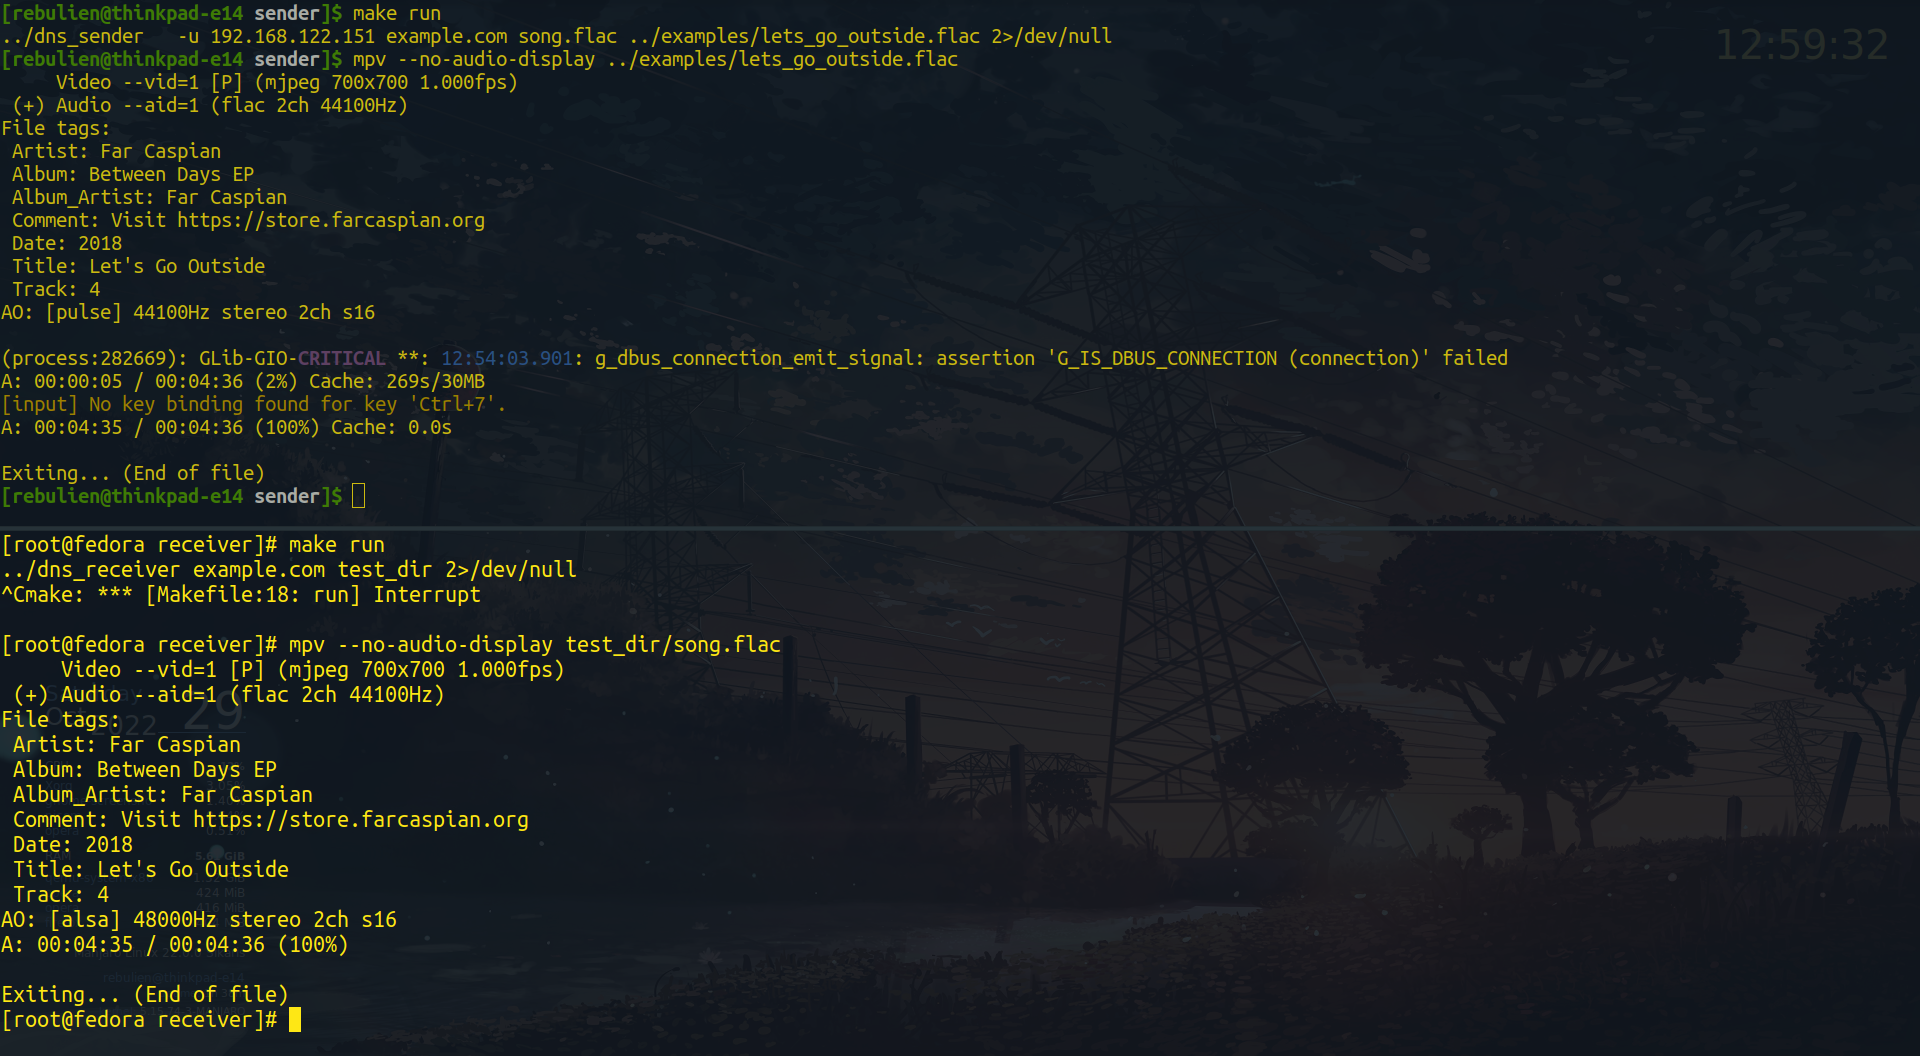
\includegraphics[width=\textwidth]{send_flac_file.png}
        \caption{Odesílání a spuštění binárního souboru (FLAC soubor)}
    \end{figure}
    \clearpage

    % zdroje
    \bibliographystyle{czechiso}
    \renewcommand{\refname}{Literatura}
    \bibliography{citace}
    \nocite{ComputerNetworking}
    \nocite{SocketProgramming}
\end{document}
